%!Tex root=./TitleI-Slides.tex
%TCIDATA{Version=5.50.0.2960}
%TCIDATA{LaTeXparent=0,0,abowd-schmutte-privacy-seminar.tex}

%TCIDATA{CSTFile=beamer.cst}

% To implement the economic approach requires a model for data publication that satisfies certain properties: (1) privacy and accuracy should be continuously measurable quantities; (2) a production function-like relationship obtains between privacy and accuracy; (3) privacy and accuracy are public goods.

% DP fits the bill. We therefore model the problem faced by a data custodian who operates a differentially private publication mechanism that yields a known menu of feasible combinations of privacy and accuracy. Given a known menu, the challenge remains to decide which combination to choose. This social choice problem requires us to separate what is feasible from what is desirable. We propose Samuelson's classic theory of public goods as a sensible place to start.

% Our effort bridges literatures from computer science, statistics, and economics [POSITION]


% What is differential privacy?


% Is differential privacy = privacy?


% **IT is important to fix ideas. Think about internment, or the existence of answers to a question on citizenship in combination with an effectively infinite set of published contingency tables.

% Database reconstruction theorem: suppose it were possible to reconstruct answers to a citizenship question together with information on block of residence. 

%%%%%%%%%%%%%%%%%%%%%%%%%%%%%%%%%%%%%%%%%%%%%%%%%%%%%%%%%%%%%%%%%
%%%%%%%%%%%%%%%%%%%%%%%%%%%%%%%%%%%%%%%%%%%%%%%%%%%%%%%%%%%%%%%%%


\section[Introduction]{Introduction}


%%%%%%%%%%%%%%%%%%%%%%%%%%%%%%%%%%%%%%%%%%%%%%%%%%%%%%%%%%%%%%%%%
%%%%%%%%%%%%%%%%%%%%%%%%%%%%%%%%%%%%%%%%%%%%%%%%%%%%%%%%%%%%%%%%%
%TCIMACRO{\TeXButton{BeginFrame}{\begin{frame}[allowframebreaks]}}%
%BeginExpansion
\begin{frame}[allowframebreaks]%
%EndExpansion
\frametitle{Problem}

{\Large Data custodians trade-off}\vspace*{.25in}
\begin{itemize}
	\item Providing detailed and accurate statistics \vspace*{.25in}
	\item Protecting privacy and confidentiality \vspace*{.5in}
\end{itemize}
{\Large What is the optimal trade-off, given that the data have already been collected?}

%TCIMACRO{\TeXButton{EndFrame}{\end{frame}}}%
%BeginExpansion
\end{frame}%
%EndExpansion
%
%%%%%%%%%%%%%%%%%%%%%%%%%%%%%%%%%%%%%%%%%%%%%%%%%%%%%%%%%%%%%%%%%
%%%%%%%%%%%%%%%%%%%%%%%%%%%%%%%%%%%%%%%%%%%%%%%%%%%%%%%%%%%%%%%%%

%%%%%%%%%%%%%%%%%%%%%%%%%%%%%%%%%%%%%%%%%%%%%%%%%%%%%%%%%%%%%%%%%
%%%%%%%%%%%%%%%%%%%%%%%%%%%%%%%%%%%%%%%%%%%%%%%%%%%%%%%%%%%%%%%%%
%TCIMACRO{\TeXButton{BeginFrame}{\begin{frame}[allowframebreaks]}}%
%BeginExpansion
\begin{frame}[allowframebreaks]%
%EndExpansion
\frametitle{Economic Approach}
% {\Large Competing uses of a finite resource: } \vspace{.25in}
\begin{enumerate}
	\item Finite resource: Information in an existing database\vspace{.25in}
	\item Competing uses:
	\begin{itemize}
		\item Statistical accuracy, versus
		\item Data privacy\vspace{.25in}
	\end{itemize}

	\item An optimal allocation should equate
	\begin{itemize}
		\item Marginal Rate of Transformation
		\item Willingness to Pay (Marginal Rate of Substitution)\vspace{.25in}
	\end{itemize}
	\item Accuracy and privacy are public goods
\end{enumerate}


%TCIMACRO{\eXButton{EndFrame}{\end{frame}}}%
%BeginExpansion
\end{frame}%
%EndExpansionT
%

%%%%%%%%%%%%%%%%%%%%%%%%%%%%%%%%%%%%%%%%%%%%%%%%%%%%%%%%%%%%%%%%%
%%%%%%%%%%%%%%%%%%%%%%%%%%%%%%%%%%%%%%%%%%%%%%%%%%%%%%%%%%%%%%%%%

%%%%%%%%%%%%%%%%%%%%%%%%%%%%%%%%%%%%%%%%%%%%%%%%%%%%%%%%%%%%%%%%%
%%%%%%%%%%%%%%%%%%%%%%%%%%%%%%%%%%%%%%%%%%%%%%%%%%%%%%%%%%%%%%%%%
%TCIMACRO{\TeXButton{BeginFrame}{\begin{frame}[allowframebreaks]}}%
%BeginExpansion
\begin{frame}[t]%
%EndExpansion
\frametitle{Social Welfare Maximization}
Social planner's problem: Maximize welfare subject to the PPF

\begin{onlyenv}<1-4>
	\begin{center}
		\includegraphics<1>[scale=.4]{blank}
		\includegraphics<2>[scale=.4]{Max_1}
		\includegraphics<3>[scale=.4]{Max_2}
		\includegraphics<4>[scale=.4]{Max_3}
		% \includegraphics<5>[scale=.4]{Max_4}
	\end{center}
\end{onlyenv}

%TCIMACRO{\TeXButton{EndFrame}{\end{frame}}}%
%BeginExpansion
\end{frame}%
%EndExpansion
%
%%%%%%%%%%%%%%%%%%%%%%%%%%%%%%%%%%%%%%%%%%%%%%%%%%%%%%%%%%%%%%%%%
%%%%%%%%%%%%%%%%%%%%%%%%%%%%%%%%%%%%%%%%%%%%%%%%%%%%%%%%%%%%%%%%%

%%%%%%%%%%%%%%%%%%%%%%%%%%%%%%%%%%%%%%%%%%%%%%%%%%%%%%%%%%%%%%%%%
%%%%%%%%%%%%%%%%%%%%%%%%%%%%%%%%%%%%%%%%%%%%%%%%%%%%%%%%%%%%%%%%%
%TCIMACRO{\TeXButton{BeginFrame}{\begin{frame}[allowframebreaks]}}%
%BeginExpansion
\begin{frame}[allowframebreaks]%
%EndExpansion
\frametitle{Today: Focus on the Demand Side}
% {\Large Competing uses of a finite resource: } \vspace{.25in}
\begin{wideitemize}
  \item Need two things to find the socially optimal point:
  \begin{enumerate}
    \item Demand for accuracy (\emph{Data Utility})
    \item Demand for privacy (\emph{Information Utility})
  \end{enumerate}
  \item Stylized application to allocation of Title I funding

\end{wideitemize}
%TCIMACRO{\eXButton{EndFrame}{\end{frame}}}%
%BeginExpansion
\end{frame}%
%EndExpansionT
%

%%%%%%%%%%%%%%%%%%%%%%%%%%%%%%%%%%%%%%%%%%%%%%%%%%%%%%%%%%%%%%%%%
%%%%%%%%%%%%%%%%%%%%%%%%%%%%%%%%%%%%%%%%%%%%%%%%%%%%%%%%%%%%%%%%%

%%%%%%%%%%%%%%%%%%%%%%%%%%%%%%%%%%%%%%%%%%%%%%%%%%%%%%%%%%%%%%%%%
%%%%%%%%%%%%%%%%%%%%%%%%%%%%%%%%%%%%%%%%%%%%%%%%%%%%%%%%%%%%%%%%%

\section{Background}
\begin{transitionframe}
  \begin{center}
    \Huge Some background
  \end{center}
\end{transitionframe}


\begin{frame}{Motivation}
  \begin{wideitemize}
    \item \emph{Database Reconstruction Theorem} and \emph{Fundamental Law of Information Recovery}
    \begin{itemize}
    	\item  \footnotesize \color{darkgray} [Dinur and Nissm (2003); Dwork, McSherry, Talwar (2007)] \color{black}\normalsize
    	\item Publication of ``too many'' statistics with ``too much'' accuracy is \emph{blatantly non-private}
    \end{itemize}
  \end{wideitemize}
\end{frame}


\begin{frame}{Model Overview}
\begin{columns}[T] % align columns
\begin{column}{.58\textwidth}
  \begin{wideitemize}
    \item Data Custodian
    \item Existing database, $D$
    \item Desired statistics, or queries, $Q$
    \item Publication mechanism: $M(D,Q)$
  \end{wideitemize}
\end{column}%
\hfill%
\begin{column}{.38\textwidth}
  \makebox[\linewidth][c]{
    \resizebox{\linewidth}{!}{
      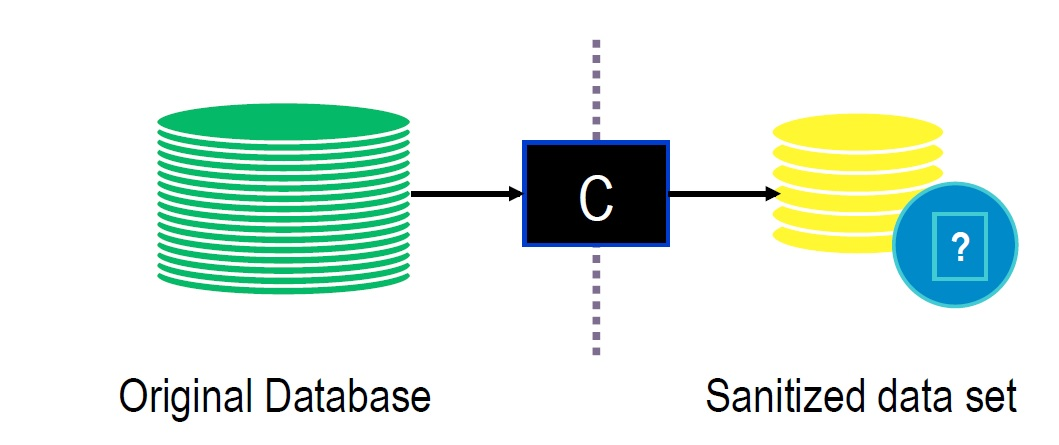
\includegraphics{privacy_dream.jpg}
    }
  }
\end{column}%
\end{columns}
\end{frame}

\begin{frame}[allowframebreaks]%
	\frametitle{Differential Privacy and Inferential Disclosure}
	Mechanism $M$ is \emph{$\varepsilon$-differentially private} if
		\begin{equation*}
		\ln\left(\frac{\Pr \left[ M(x,Q)\in B \ |x,Q\right]}{\Pr \left[
			M(x^{\prime },Q)\in B \ |x^{\prime},Q\right]}\right)
			 \leq \varepsilon 
	    \end{equation*}%
	 \footnotesize \color{darkgray} 
	 \color{black}\normalsize \\
	 \ \\
	\textbf{Properties}
	\begin{wideitemize}
	    \item \emph{Data reconstruction:} $\varepsilon$ bounds change in output from changing input
	    \item \emph{Privacy loss:} $\varepsilon$ bounds ``worst-case'' update about $x$
	    \item \emph{Composes:} Losses due to multiple uses of the same data are ``added up''
	    \item \emph{Future Proof:} Guarantees independent of outside knowledge
	    \item \emph{Public:} Mechanism and parameters can be published [\emph{SDL-aware analysis}]
	\end{wideitemize}
\end{frame}%

\begin{frame}[allowframebreaks]%
  \frametitle{Defining Accuracy}
  % We define accuracy in terms of the squared $\ell_2$ distance between the mechanism output and the exact answer $Q(x)$.
\begin{definition}[Accuracy ($I$)]
  \label{def:accuracy}
  Given histogram $x \in \mathbb{Z}^{\ast |\chi |}$ and query workload $Q \in  \mathcal{F}$, the data publication mechanism $M(x,Q)$ has accuracy $I$ if
  $$\mathbb{E}\left[\left\Vert(M(x,Q) - Q(x)\right\Vert^{2}_{2}\right] = -I.$$ where $I\le 0$ and the expectation is taken only over the randomness in $M(x,Q)$.
\end{definition}
\begin{wideitemize}
  \item $\left\Vert\cdot\right\Vert^{2}_{2}$ is the square of the $\ell_{2}$ distance.
  \item expectations taken over the distn.\ induced by $M(x,Q)$.
\end{wideitemize}
%In this definition, .

\end{frame}%

\begin{frame}[allowframebreaks]%
  \frametitle{Differential Privacy as Production Technology}
  We argue that some DP mechanisms are proper production technologies: $X$-efficient for accuracy, given privacy loss
\vskip.25in
  {\Large\textbf{Examples:}}
  \begin{wideitemize}
    \item \emph{Randomized Response}
    \item \emph{Laplace Mechanism}
    \item \emph{Matrix Mechanism}
  \end{wideitemize}
\end{frame}%

\begin{frame}[allowframebreaks]%
  \frametitle{Laplace Mechanism}
  \begin{theorem}[Laplace Mechanism]
  \label{prop:laplace_mechanism}
   For $\varepsilon>0$, query workload $Q$, and histogram $x$, define data publication mechanism
   $\limfunc{Lap}(x,Q) \equiv Qx + e$,
   where $e$ is a conformable vector of iid samples drawn from the Laplace distribution with scale parameter
   $b=\frac{\Delta Q }{\varepsilon}$.
   $Lap(x,Q)$ is $\varepsilon$-differentially private.
\end{theorem}
\begin{wideitemize}
  \item $\Delta Q$ is sensitivity of the query workload
  \item Data indepedent
  \item Yields a concave production relationship:
  $$ I = -\frac{2L\left(\Delta Q\right)^{2}}{\varepsilon^{2}}$$
  when $L$ is the total number of queries
\end{wideitemize}
\end{frame}%


%%%%%%%%%%%%%%%%%%%%%%%%%%%%%%%%%%%%%%%%%%%%%%%%%%%%%%%%%%%%%%%%%
%%%%%%%%%%%%%%%%%%%%%%%%%%%%%%%%%%%%%%%%%%%%%%%%%%%%%%%%%%%%%%%%%

\section{Application to Title I Funding}
\begin{transitionframe}
  \begin{center}
    \Huge Application to Title I
  \end{center}
\end{transitionframe}

\begin{frame}{Setting}
  \begin{wideitemize}
    \item Title I funds appropriated by Congress to needy school districts
    \item DOE allocates to district $\ell$ using 
$$
	A_{\ell} = E_{\ell}\times C_{\ell},
$$
    \begin{itemize}
    	\item $A_{\ell}$ is the \emph{authorization amount}
    	\item $E_{\ell}$ is the \emph{eligibility count}
    	\item $C_{\ell}$ is the \emph{adjusted per-pupil expenditure}
    \end{itemize}
    \item Census publishes $\widehat{E}_{\ell}$
    \item \textbf{Target Allocation:} $X = \sum_{\ell=1}^{L} E_{\ell}\times C_{\ell}$
    \item \textbf{Actual Allocation:} $\widehat{X} = \sum_{\ell=1}^{L} \widehat{E}_{\ell}\times C_{\ell}$
  \end{wideitemize}
  {\textbf{Policy challenge:} balance privacy loss among disadvantaged households against misallocation of Title I funds}
\end{frame}

\begin{frame}{Publication Mechanism}
  \begin{wideitemize}
  	\item \textbf{Database:} Households with indicator for Title I eligibility and district geocode
  	\item \textbf{Queries:} Count of Title I households by district ($E_{\ell}$)
  	\item \textbf{Mechanism:} Laplace Mechanism (Matrix Mechanism)
  	\begin{itemize}
  		\item Publish $\widehat{E}_{\ell} = E_{\ell}+e_{\ell}$ 
  		\item $e_{\ell}$ is Laplace noise with scale parameter $\varepsilon^{-1}$
  		\item Satisfies $\varepsilon-$differential privacy
  		\item Accuracy:
			$$
				I = -\mathbb{E}\left[\sum_{\ell=1}^{L}\left(\widehat{E}_{\ell}-E_{\ell}\right)^{2}\right] = -\frac{2L}{\varepsilon^{2}}
			$$
  	\end{itemize}
  \end{wideitemize}
\end{frame}

\begin{frame}{Social Welfare Function}
\begin{equation*}
  SWF = \phi\sum_{i}v_{i}^{Info}(\varepsilon) + (1-\phi)v^{Data}(I),
\end{equation*}
  \begin{wideitemize}
    \item Weight, $0\le\phi\le1$, on privacy preferences
    \item \textbf{Information Utility:} $v_{i}^{Info}(\varepsilon) = -k_{i}\varepsilon$
    \item \textbf{Data Utility:} $v^{Data}(I) = a_{i} + b_{i} I$

  \end{wideitemize}
\end{frame}



%%%%%%%%%%%%%%%%%%%%%%%%%%%%%%%%%%%%%%%%%%%%%%%%%
%Preferences for privacy
\begin{transitionframe}
  \begin{center}
    \Huge Information Utility
  \end{center}
\end{transitionframe}

\begin{frame}{Information Utility}
  (based on Ghosh and Roth [2015])
  \begin{wideitemize}
    \item Let $\Omega$ be a set of future states that can be affected by disclosure \ \\
    e.g., identity theft; denial of health insurance; persecution
    \item Utility: $u_{i}(\omega)$ with $\omega\in\Omega$
    \item Mechanism: $M(x,Q)$ has output drawn from $\mathcal{R}$ 
    \item $M(x,Q)$ is $\varepsilon$-differentially private
  \end{wideitemize}

\end{frame}

\begin{frame}{Information Utility}
  \begin{wideitemize}
    \item Let $z:\mathcal{R}\rightarrow\Delta\Omega$ map mechanism output to probabilities of future states
    \item Question: How much worse off is $i$ when her data is included in $x$ versus when it is excluded?
    \item Claim: Mechanism $Z(x,Q) = z(M(x,Q))$ is $\varepsilon$-differentially private 
    \item Let $x^\prime$ be a neighboring database that excludes $i$'s data   
  \end{wideitemize}
  It follows that
$$\mathbb{E}_{\omega|M(x,Q)}\left[u_{i}(\omega)\right] \le e^{\varepsilon}\mathbb{E}_{\omega|M(x^\prime,Q)}\left[u_{i}(\omega)\right]$$
  Worst case incremental utility change is:
  $$\Delta U = \left(e^{\varepsilon}-1\right)k_{i}$$ 
  $k_{i}$ is expected utility over future events when $i$'s data are \emph{not} included in the mechanism.\ \\
  When $\varepsilon \approx 0$
  $$\left(e^{\varepsilon}-1\right)k_{i}\approx\varepsilon k_{i}$$
\end{frame}

%%%%%%%%%%%%%%%%%%%%%%%%%%%%%%%%%%%%%%%%%%%%%%%%%
%Preferences for privacy
\begin{transitionframe}
  \begin{center}
    \Huge Data Utility
  \end{center}
\end{transitionframe}

\begin{frame}{Data Utility}
  \textbf{Result:} reduced-form linear in accuracy: $v^{data}_{i}(I) =  a_{i} + b_{i}I$
  \begin{wideitemize}
    \item utility from wealth: $U_{i}(W_{i})$ (strictly concave)
    \item $W_{i} = \Pi_{i}^{T} M(x,Q)$ 
    \begin{itemize}
      \item $M(x,Q) = Qx + e$ is Laplace mechanism
      \item $\Pi_{i}$ is a vector of weights
    \end{itemize} 
  \end{wideitemize}

  
\end{frame}

\begin{frame}{Data Utility}
 Expected utility for any person $i$ is
$$
  \mathbb{E}\left[U_{i}(W_{i})\right] = \mathbb{E}_{x}\left[\mathbb{E}_{e|x}\left[U_{i}\left(\Pi_{i}^{T}Qx + \Pi_{i}^{T}e\right)\vert x\right] \right].
$$
approximated as
 \begin{equation}
  \begin{array}{rcl}
   \mathbb{E}\left[U_{i}(W_{i})\right]  \approx &  \mathbb{E}_{x}\left[U_{i}(\Pi_{i}^{T}Qx)\right] &- I\cdot \left\{\frac{1}{2}\mathbb{E}_{x}\left[U_{i}^{\prime\prime}(\Pi_{i}^{T}Qx)\right] \frac{\left\Vert \Pi_{i}^{T} \right\Vert^{2}}{L}\right\} \\
   \equiv & a_{i} & + I\cdot b_{i}.
   \end{array}
 \end{equation}
 \end{frame}
  
%%%%%%%%%%%%%%%%%%%%%%%%%%%%%%%%%%%%%%%%%%%%%%%%%
%Preferences for privacy
\begin{transitionframe}
  \begin{center}
    \Huge Back to the Title I Application
  \end{center}
\end{transitionframe}

\begin{frame}{Social Welfare Function}
\begin{equation*}
  SWF = \phi\sum_{i}v_{i}^{Info}(\varepsilon) + (1-\phi)v^{Data}(I),
\end{equation*}
  \begin{wideitemize}
    \item Weight, $0\le\phi\le1$, on privacy preferences
    \item \textbf{Information Utility:} $v_{i}^{Info}(\varepsilon) = -k_{i}\varepsilon$ %[\citet{Ghosh:Auction:GEB:2015}]
    \item \textbf{Data Utility:} $v^{Data}(I)$
      \begin{itemize}
        \item Linear-quadratic in aggregate misallocation: $W=(\widehat{X}-X) = \sum_{\ell=1}^{L}C_{\ell}\left[\widehat{E}_{\ell}-E_{\ell}\right]$
        \item $v^{Data}(I)=I\sum_{\ell=1}^{L}\frac{C_{\ell}^{2}}{L}$
      \end{itemize}
  \end{wideitemize}
\end{frame}


\begin{frame}{Calibration}
\begin{columns}[T] % align columns
\begin{column}{.58\textwidth}
		\begin{equation*}
			WTA \equiv \frac{dI}{d\varepsilon} = \left(\frac{\phi}{1-\phi}\right) N\frac{\bar{k}}{\bar{C^{2}}},
		\end{equation*}
  \begin{wideitemize}
    \item $L=13,000$ public school districts
    \item $N=46$ million school-age children
    \item average squared spending, $\bar{C^{2}}\approx 20$ million
    \item $\bar{k}=\$1,400$ (avg.\ cost of identity theft)
    \item Setting $WTA = MRT$ 
      $$\varepsilon = 2.52\times \left(\frac{\phi}{1-\phi}\right)^{-\frac{1}{3}}$$
  \end{wideitemize}
\end{column}%
\hfill%
\begin{column}{.38\textwidth}
  \makebox[\linewidth][c]{
    \resizebox{\linewidth}{!}{
      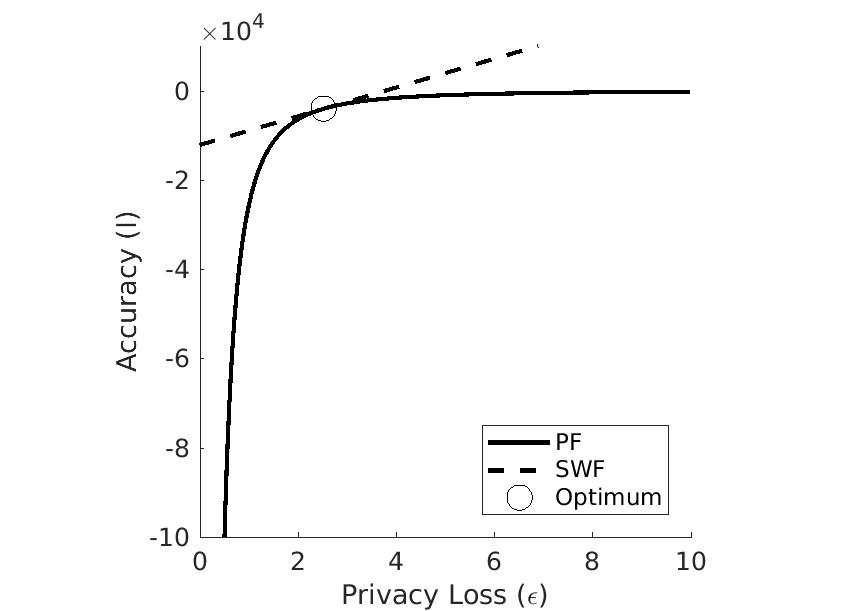
\includegraphics{plannersprob.jpg}
    }
  }
\end{column}%
\end{columns}
\end{frame}

\begin{frame}[fragile]{Calibration}
\begin{columns}[T] % align columns
\begin{column}{.58\textwidth}
  $$\eta = \frac{\phi}{1-\phi}$$
  \begin{wideitemize}
    \item<1-> $\eta=1$
    \begin{itemize}
    	\item<2->  $\varepsilon^{\ast}=2.52$
    	\item<2->  $RMSE:$ \$2,509 (70 cents per student)
    \end{itemize}
    \item<3-> $\eta= \frac{N}{POP-N}\approx 0.15$
    \begin{itemize}
    	\item<4-> $\varepsilon^{\ast\ast} = 4.74$
    	\item<4-> $RMSE:$ \$1,334 (38 cents per student)
    \end{itemize}
    \item<5-> Privacy advocates urge $\varepsilon<<1$
    \begin{itemize}
    	\item<6-> Fix $\varepsilon=0.1$
    	\item<6-> $RMSE: $\$63,000 (\$18 per student)
    \end{itemize}
  \end{wideitemize}
\end{column}%
\hfill%
\begin{column}{.38\textwidth}
  \makebox[\linewidth][c]{
    \resizebox{\linewidth}{!}{
      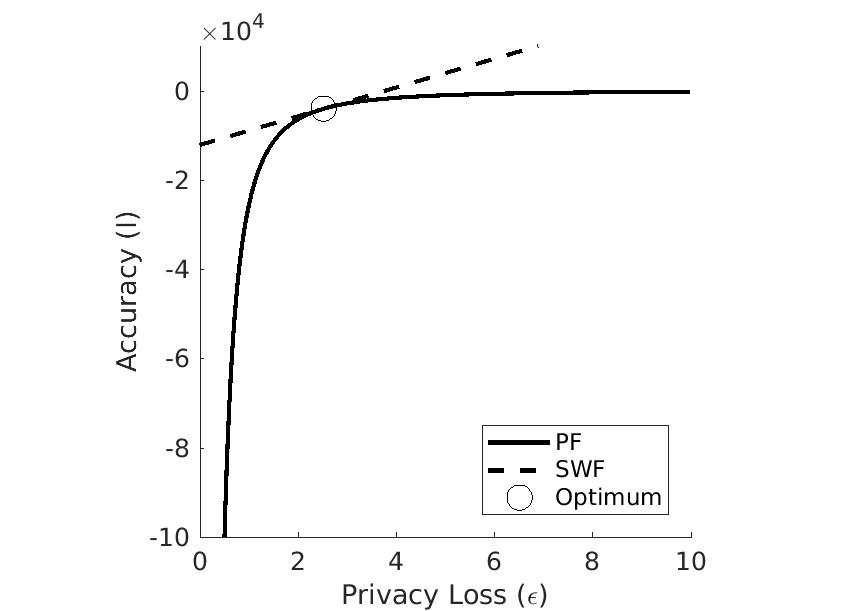
\includegraphics{plannersprob.jpg}
    }
  }
\end{column}%
\end{columns}
\end{frame}

%%%%%%%%%%%%%%%%%%%%%%%%%%%%%%%%%%%%%%%%%%%%%%%%%
%Other applications
\begin{transitionframe}
  \begin{center}
    \Huge Other Applications
  \end{center}
\end{transitionframe}

\begin{frame}{Legislative Redistricting}
  \begin{wideitemize}
    \item Data utility is based on
    \begin{itemize}
        \item Supreme Court one-person one-vote decision (all legislative districts must have approximately equal populations; there is judicially approved variation)
        \item Statistical disclosure limitation is a “statistical method” (permitted by Utah v. Evans) not “sampling” (prohibited by the Census Act, confirmed in Commerce v. House of Representatives)
        \item Voting Rights Act, Section 2: requires majority-minority districts at all levels, when certain criteria are met
    \end{itemize}
    \item The privacy utility is based on
    \begin{itemize}
        \item Title 13 requirement not to publish exact identifying information
        \item The public policy implications of uses of race, ethnicity and citizenship tabulations at detailed geography
    \end{itemize}
  \end{wideitemize}
\end{frame}

\begin{frame}{Economic Censuses and National Accounts}
  \begin{wideitemize}
    \item The major client is the producer of national accounts
    \item In most countries these activities are consolidated in a single agency
    \item Data utility: accuracy of the national accounts
    \item Privacy utility: sensitivity of detailed industry and product data
    \item Detailed tables can be produced using formal privacy with far less suppression bias than in current methods
    \item But it's an inefficient use of the global privacy-loss budget when the accounts are published at much more aggregated levels
    \item Optimize the data and privacy utility trade-offs by sharing confidential data (as permitted under CIPSEA) and applying formal privacy at publication level
  \end{wideitemize}
\end{frame}

\begin{frame}{Tax Data and Tax Simulations}
  \begin{wideitemize}
    \item Simulating the effects of tax policy changes is an important use of tax micro-data
    \item Traditional disclosure limitation methods aggravate these simulations by smoothing over important kinks and breaking audit consistency
    \item Data utility: quality of the simulated tax policy effects
    \item Privacy utility: sensitivity of the income tax returns
    \item Detailed tables can be produced using formal privacy with far less suppression bias than in current methods
    \item But it's an inefficient use of the global privacy-loss budget when the accounts are published at much more aggregated levels
    \item Optimize the data and privacy utility trade-offs by doing the simulations inside the IRS firewall and applying formal privacy protection to outputs
  \end{wideitemize}
\end{frame}

\begin{frame}{General Purpose Public-use Micro-data}
  \begin{wideitemize}
    \item Hierarchy of users
    \begin{itemize}
        \item Educational
        \item Commercial
        \item Scientific
    \end{itemize}
    \item Data utility: valid scientific inferences on arbitrary hypotheses estimable within the design of the confidential data product 
    \item Privacy utility: reconstruction-abetted re-identification attacks make every variable a potential identifier, especially in combination
    \item Traditional SDL fails the data utility condition
    \item Formal privacy guarantees the data utility for hypotheses in the query workload--serves educational and commercial users well
    \item Other scientific hypotheses may require restricted-access to the micro-data and specialized analysis software
  \end{wideitemize}
\end{frame}

\begin{transitionframe}
  \begin{center}
    \Huge Thank  you
  \end{center}
    \begin{center}
    John.Maron.Abowd@census.gov
  \end{center}

\end{transitionframe}
%%%%%%%%%%%%%%%%%%%%%%%%%%%%%%%%%%%%%%%%%%%%%%%%%%%%%%%%%%%%%%%%%
%%%%%%%%%%%%%%%%%%%%%%%%%%%%%%%%%%%%%%%%%%%%%%%%%%%%%%%%%%%%%%%%%



%%%%%%%%%%%%%%%%%%%%%%%%%%%%%%%%%%%%%%%%%%%%%%%%%%%%%%%%%%%%%%%%%
%%%%%%%%%%%%%%%%%%%%%%%%%%%%%%%%%%%%%%%%%%%%%%%%%%%%%%%%%%%%%%%%%

\appendix

\begin{transitionframe}
  \begin{center}
    \Huge Appendix Slides
  \end{center}
\end{transitionframe}

\section{Data Publication Model}
\begin{transitionframe}
  \begin{center}
    \Huge Data Publication Model
  \end{center}
\end{transitionframe}



\begin{frame}{Database}
\begin{columns}[T] % align columns
\begin{column}{.58\textwidth}
  \begin{wideitemize}
	  \item Custodian holds a database matrix, $D$
	  \item Rows of $D$ are for $N$ individuals
	  \item Columns record variables / features.
	  \item Each column is drawn from a finite-valued \emph{data domain}, $\chi$
  \end{wideitemize}

  % {\Large Histogram Representation}
  
  % \begin{wideitemize}
	 %  \item The \emph{histogram representation} of $D$, $x \in  \mathbb{Z}^{\ast |\chi |}$
	 %  \item For each $k\in\chi$, $x_{k}$ is the number of records in $D$ with attribute combination $k$.
  % \end{wideitemize}
\end{column}%
\hfill%
\begin{column}{.38\textwidth}
  \makebox[\linewidth][c]{
    \resizebox{\linewidth}{!}{
      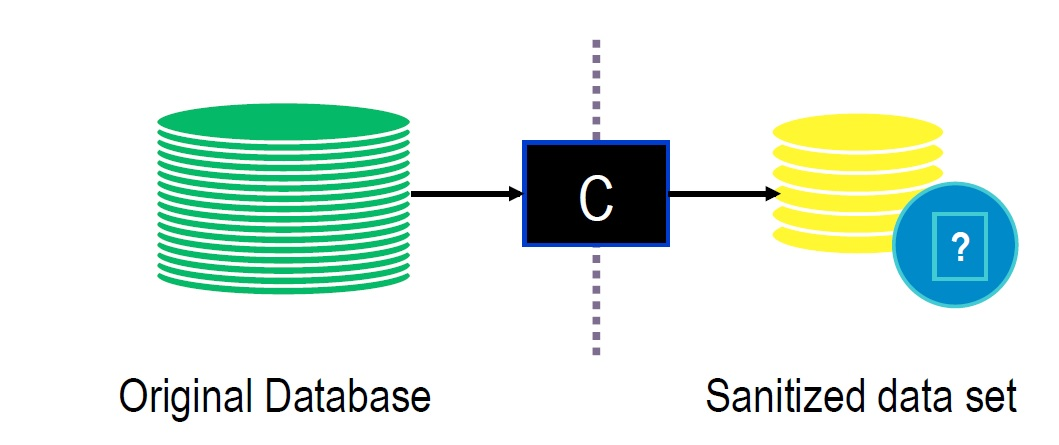
\includegraphics{privacy_dream.jpg}
    }
  }
\end{column}%
\end{columns}
\end{frame}

\begin{frame}{Queries}
\begin{columns}[T] % align columns
\begin{column}{.58\textwidth}
  \begin{wideitemize}
	  \item \emph{database query} is $q:\mathbb{Z}^{\ast |\chi |}\rightarrow \mathcal{R}$
	  \item $q(x)$ is the \emph{exact query answer}
	  \item \emph{query workload}, $Q=\{q_{1},\ldots,q_{k} \}$.
	  \item The $\ell_{1}$ sensitivity for query $q$ 
		\begin{definition}[$\ell_{1}$ Query Sensitivity]
			\label{def:query_sensitivity}
			\begin{equation*}
				\Delta q = \max_{x,y\in \mathbb{Z}^{\ast |\chi |}, \left\Vert{x}-{y}\right\Vert_{1} \le 1}|q(x)-q(y)|.
			\end{equation*}
		\end{definition}
  \end{wideitemize}
\end{column}%
\hfill%
\begin{column}{.38\textwidth}
  \makebox[\linewidth][c]{
    \resizebox{\linewidth}{!}{
      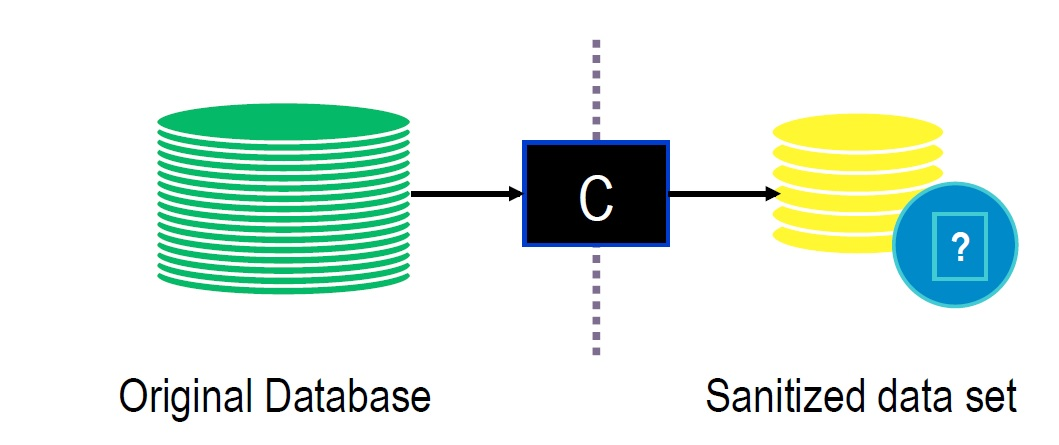
\includegraphics{privacy_dream.jpg}
    }
  }
\end{column}%
\end{columns}
\end{frame}

\begin{frame}{Data Publication Mechanism}
\begin{columns}[T] % align columns
\begin{column}{.58\textwidth}
	\begin{definition}[Data Publication Mechanism]
	\label{def:query_mechanism} Let $\mathcal{F}$ be the set of allowable query workloads.
	A \emph{data publication mechanism} is a random function
	$M:\mathbb{Z}^{\ast |\chi|}\times \mathcal{F}\rightarrow \mathcal{R}$ whose
	inputs are a histogram $x\in \mathbb{Z}^{\ast |\chi |}$ and a workload $Q \in  \mathcal{F}$,
	and whose random output is an element of range $\mathcal{R}$.
	For  $B \in \mathcal{B}$, where $\mathcal{B}$ are the measurable subsets of $\mathcal{R}$,
	the conditional probability is $\Pr \left[ M(x,Q)\in B | x,Q \right] $, given $x$ and $Q$, where
	the probabilities are over the randomness induced by the mechanism.
	\end{definition}
\end{column}%
\hfill%
\begin{column}{.38\textwidth}
  \makebox[\linewidth][c]{
    \resizebox{\linewidth}{!}{
      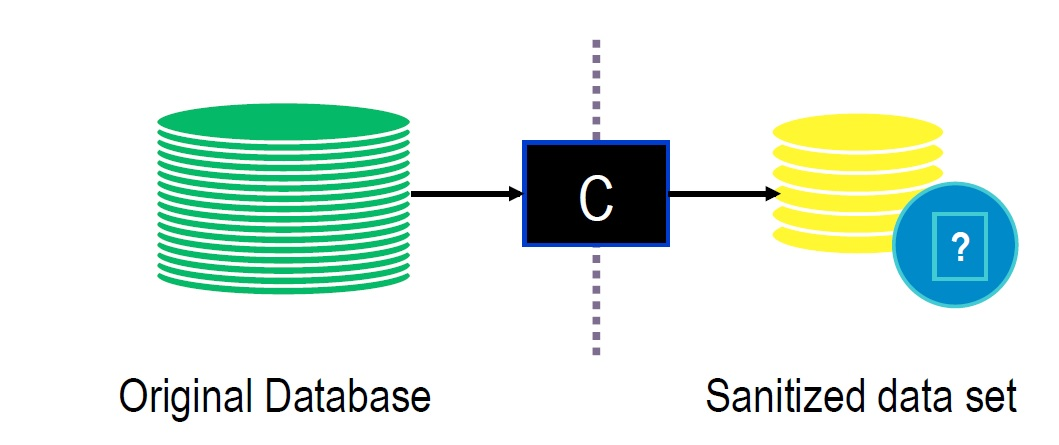
\includegraphics{privacy_dream.jpg}
    }
  }
\end{column}%
\end{columns}
\end{frame}

\section{Production}
\begin{transitionframe}
  \begin{center}
    \Huge Production Possibilities
  \end{center}
\end{transitionframe}

\begin{frame}{Defining Production}
\begin{columns}[T] % align columns
\begin{column}{.58\textwidth}
  \begin{wideitemize}
    \item Differential privacy, $\varepsilon$
    \item Data accuracy, $I$
    \item Transformation sets
  \end{wideitemize}
\end{column}%
\hfill%
\begin{column}{.38\textwidth}
  \makebox[\linewidth][c]{
    \resizebox{\linewidth}{!}{
      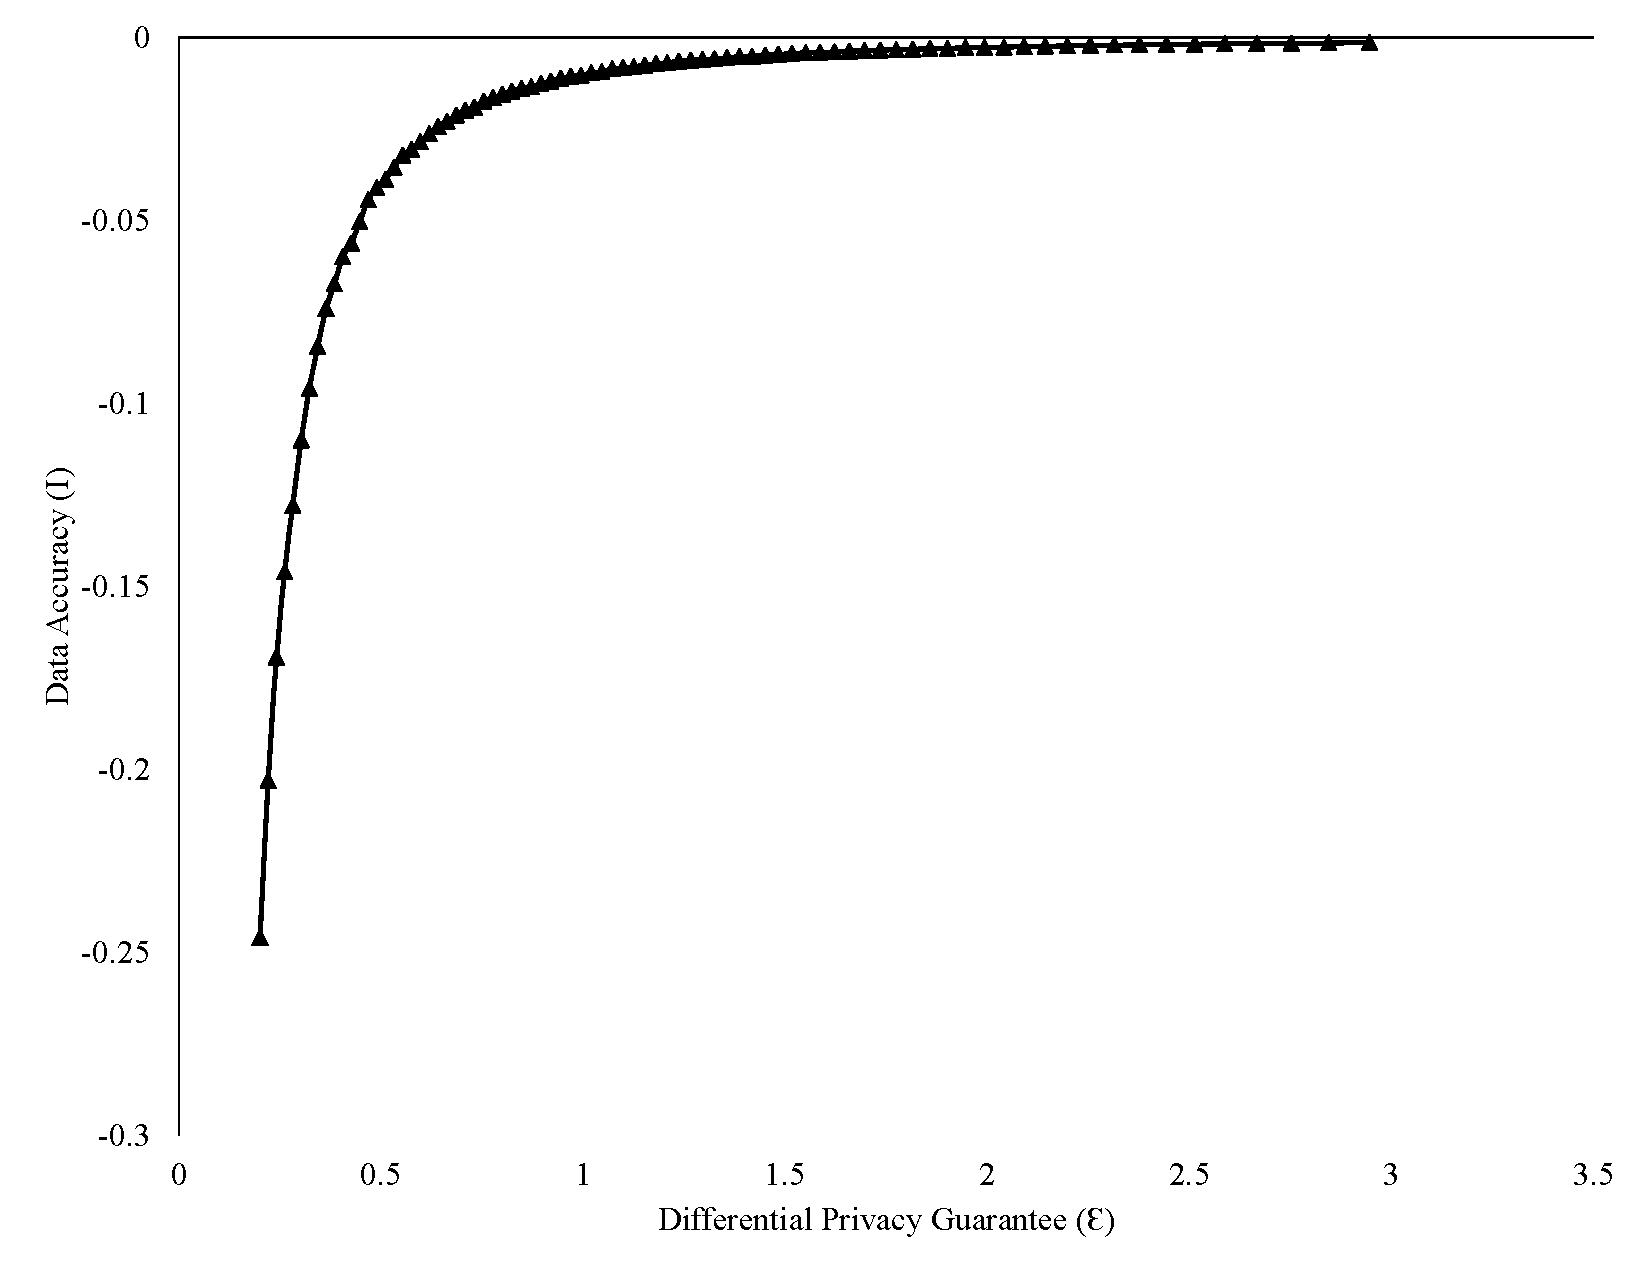
\includegraphics{RandResponse_Plot.pdf}
    }
  }
\end{column}%
\end{columns}
\end{frame}

\begin{frame}{Differential Privacy}
\begin{columns}[T] % align columns
\begin{column}{.58\textwidth}
Mechanism $M$ is \emph{$\varepsilon$-differentially private} if
	\begin{wideitemize}
		\item For all neighboring $x,x^{\prime}$, $Q$, and $B$
		\begin{equation*}
		\ln\left(\frac{\Pr \left[ M(x,Q)\in B \ |x,Q\right]}{\Pr \left[
			M(x^{\prime },Q)\in B \ |x^{\prime},Q\right]}\right)
			 \leq \varepsilon 
	    \end{equation*}%
	\end{wideitemize}
\end{column}%
\hfill%
\begin{column}{.38\textwidth}
  \makebox[\linewidth][c]{
    \resizebox{\linewidth}{!}{
      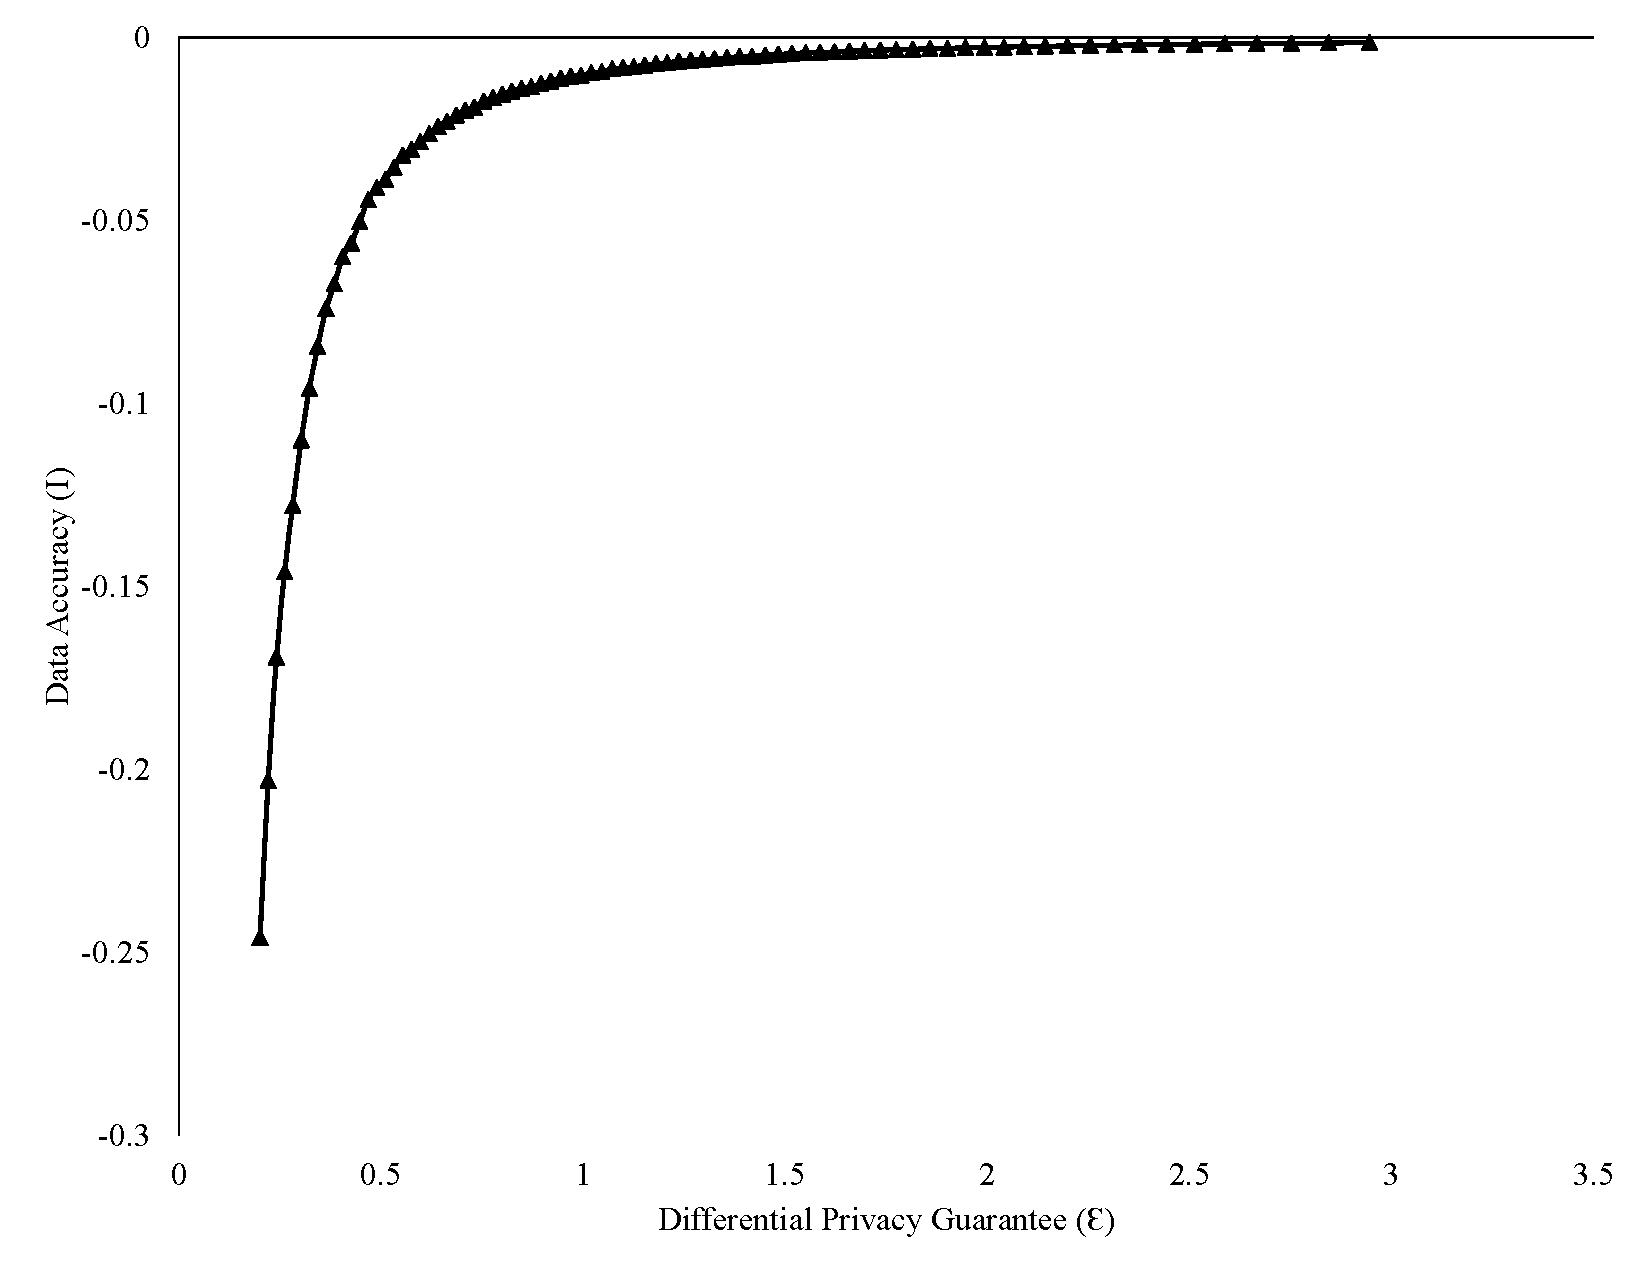
\includegraphics{RandResponse_Plot.pdf}
    }
  }
\end{column}%
\end{columns}
\end{frame}

\begin{frame}{Data Accuracy}
\begin{columns}[T] % align columns
\begin{column}{.58\textwidth}
	\begin{wideitemize}
	    \item Mechanism $M$ has accuracy $I<0$ if
	     $$\mathbb{E}\left[\left\Vert(M(x,Q) - Q(x)\right\Vert^{2}_{2}\right] = -I.$$
	     \item $\left\Vert\cdot\right\Vert^{2}_{2}$ is the square of the $\ell_{2}$ (Euclidean) distance.
	\end{wideitemize}

\end{column}%
\hfill%
\begin{column}{.38\textwidth}
  \makebox[\linewidth][c]{
    \resizebox{\linewidth}{!}{
      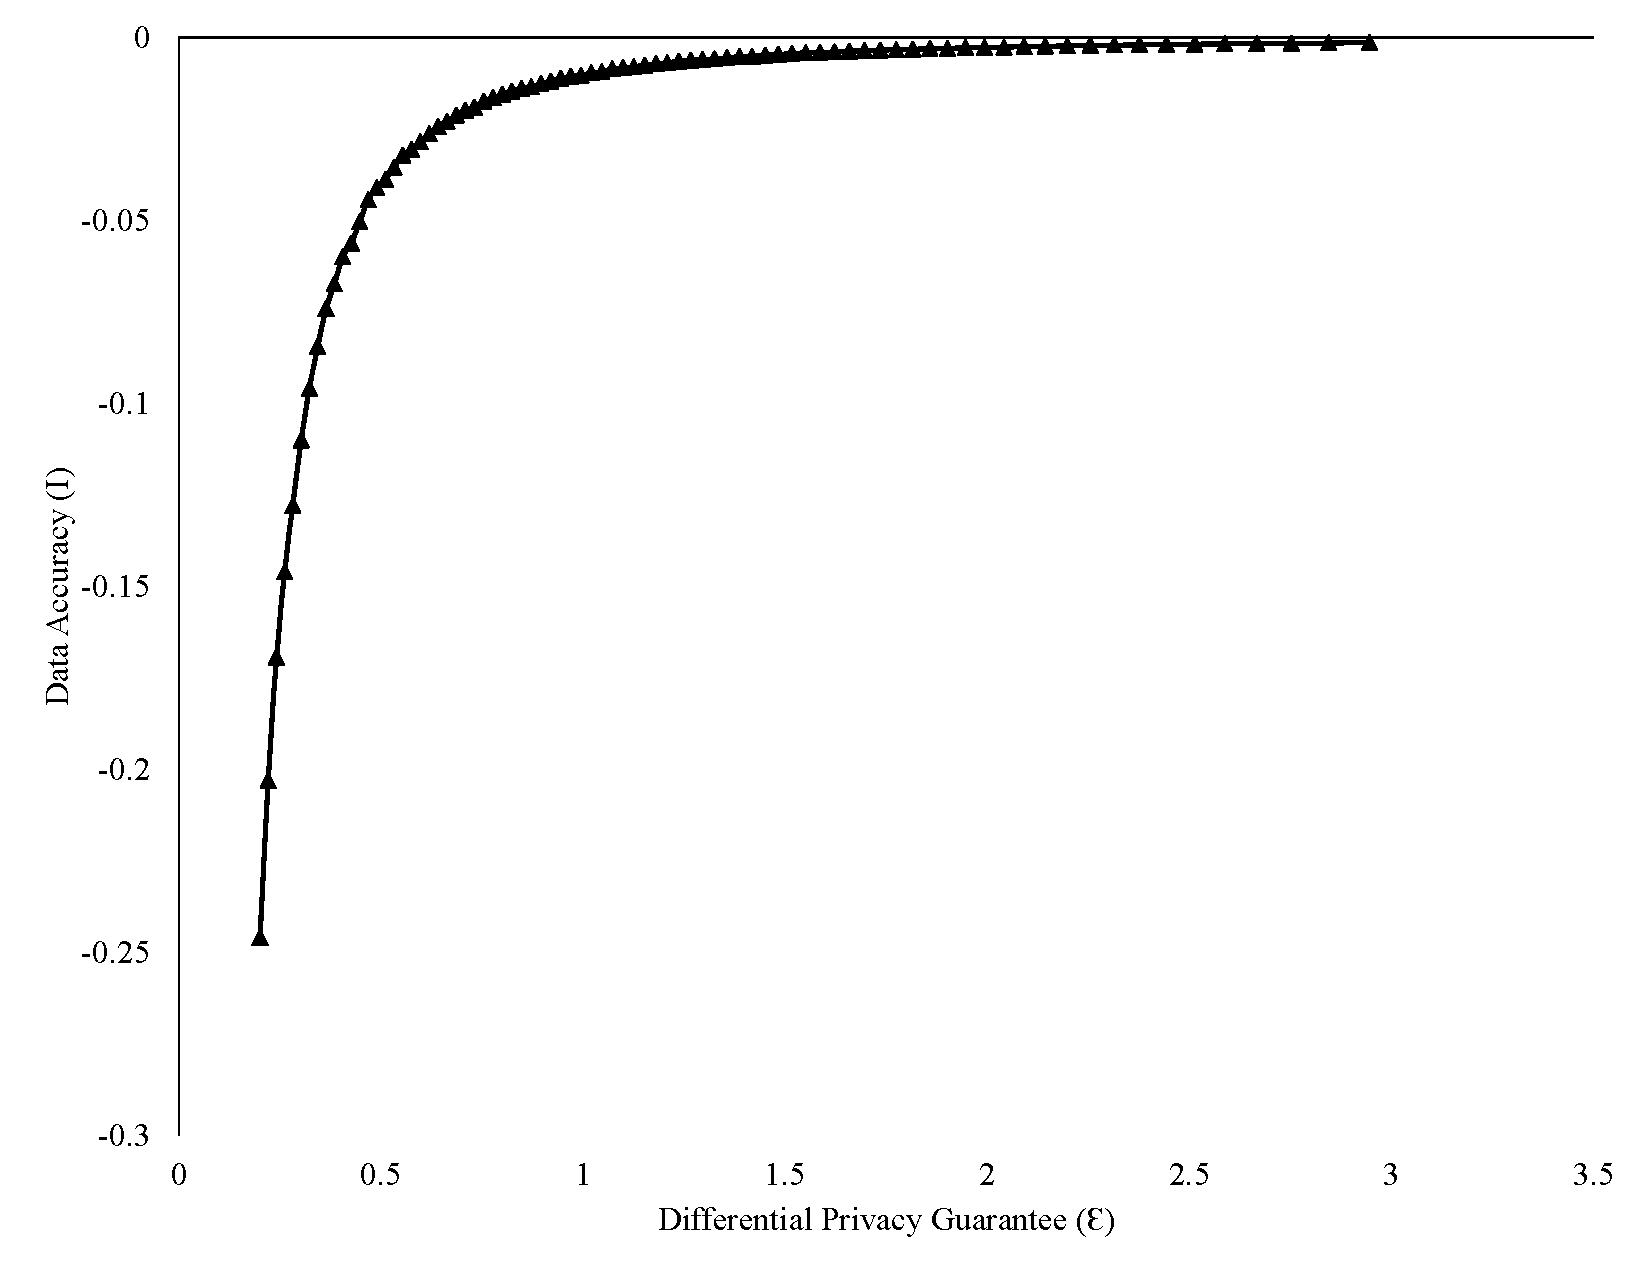
\includegraphics{RandResponse_Plot.pdf}
    }
  }
\end{column}%
\end{columns}
\end{frame}

\begin{frame}[allowframebreaks]{Transformation Sets}
\begin{columns}[T] % align columns
\begin{column}{.58\textwidth}
	\begin{wideitemize}
	    \item Each mechanism, $M$, has associated \emph{production activity} $(\varepsilon,I)$
	    \item Custodian's \emph{transformation set},
	    $$Y=\left\{ \left( \varepsilon ,I \right) \left\vert \varepsilon >0,I<0 \right. \right\}$$
	    \item \textbf{Assumptions}
	    \begin{itemize}
	    	\item $Y$ is closed and bounded
	    	\item no free lunch [\citet{Dwork2004}, \citet{Dwork2008}, \citet{gehrke2011towards}, \citet{Kifer:2011:NFL:1989323.1989345}]
	    \end{itemize}
	 %    \item \emph{transformation function} $G(\varepsilon,I)$
		% $
		% Y=\left\{ \left( \varepsilon ,I \right) \left\vert \varepsilon >0,I<0 \text{ s.t. }G(\varepsilon ,I)\leq0
		% \right\}\right\}.
		% $
		\item The \emph{production frontier}
		$$
		PF=\left\{ \left( \varepsilon ,I\right)
		\left\vert \varepsilon >0,I<0\text{ s.t. }G(\varepsilon ,I)=0\right.
		\right\}
		$$
	\end{wideitemize}
\end{column}%
\hfill%
\begin{column}{.38\textwidth}
  \makebox[\linewidth][c]{
    \resizebox{\linewidth}{!}{
      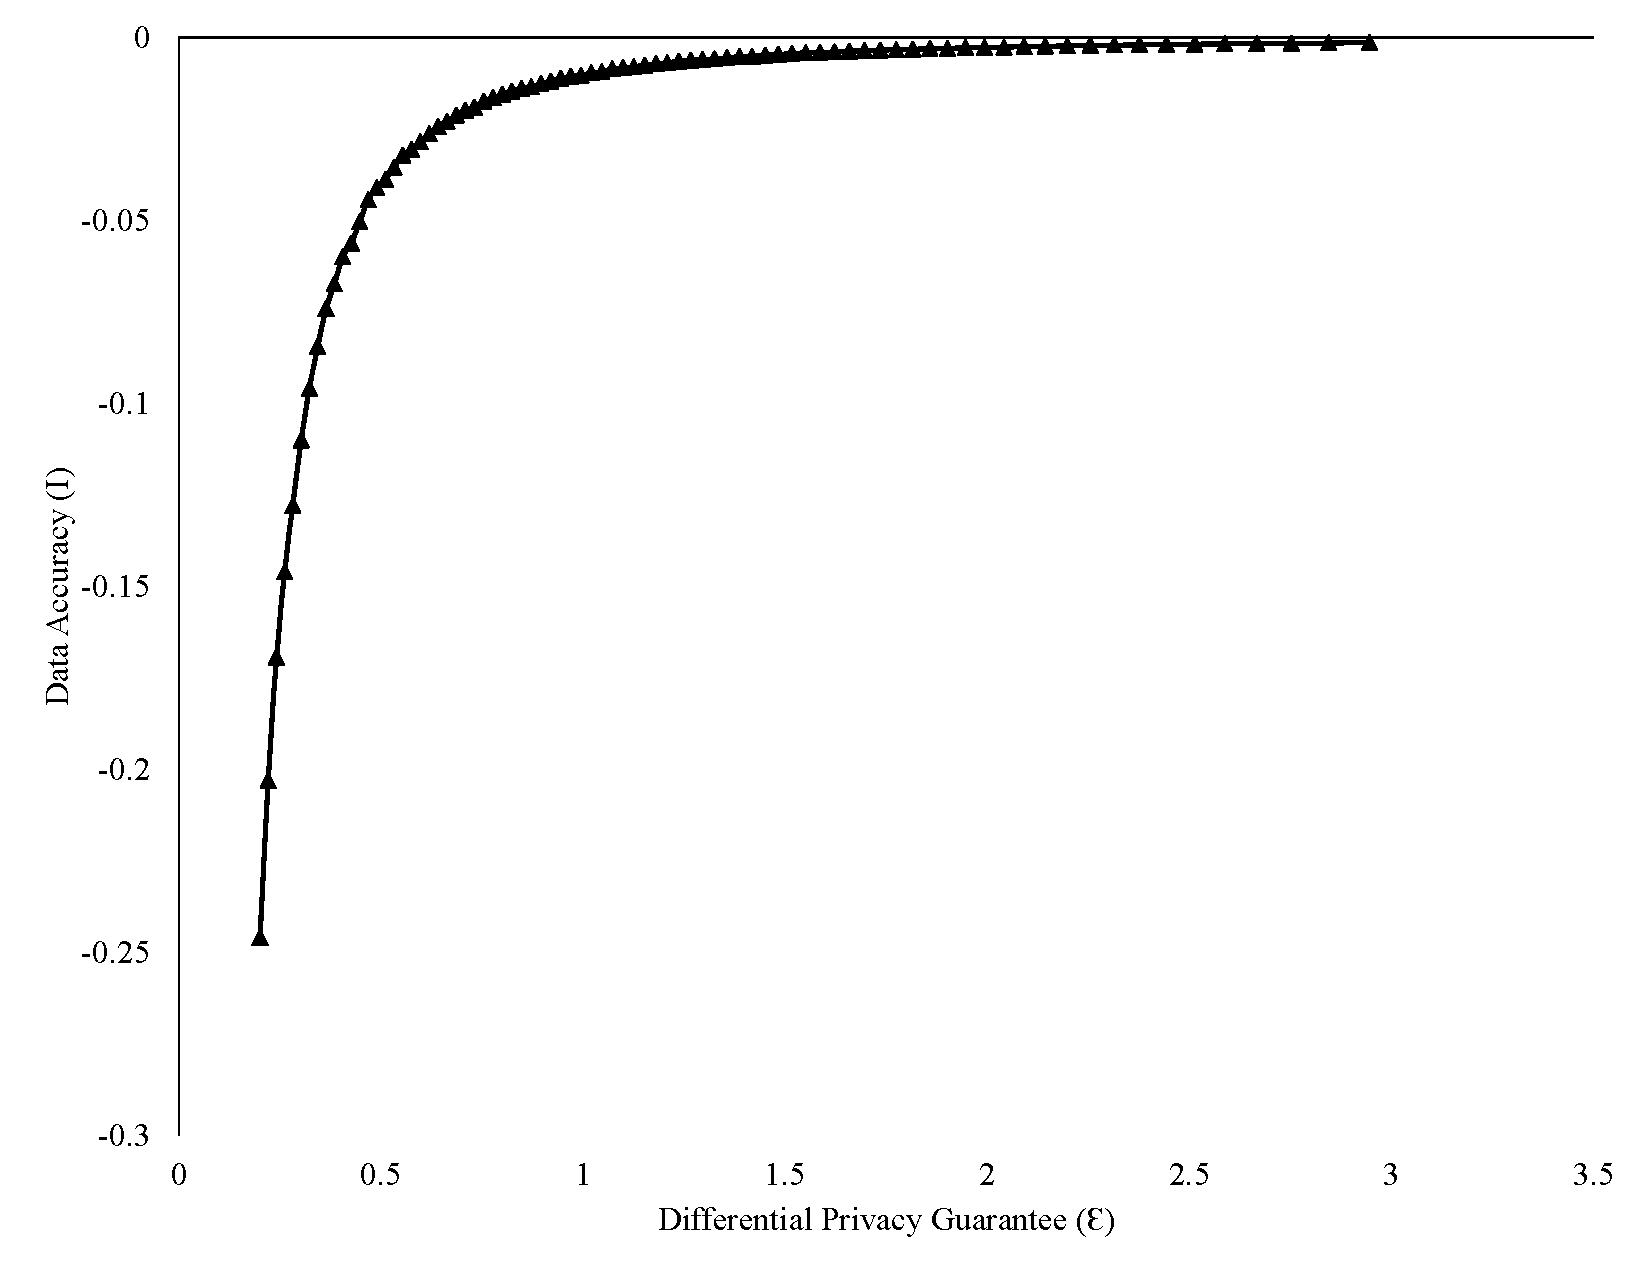
\includegraphics{RandResponse_Plot.pdf}
    }
  }
\end{column}%
\end{columns}
\end{frame}


%%%%%%%%%%%%%%%%%%%%%%%%%%%%%%%%%%%%%%%%%%%%%%%%%%%%%%%%%%%%%%%%%
%%%%%%%%%%%%%%%%%%%%%%%%%%%%%%%%%%%%%%%%%%%%%%%%%%%%%%%%%%%%%%%%%
